\begin{figure}[b]
    \centering
    \rotatebox{-90}{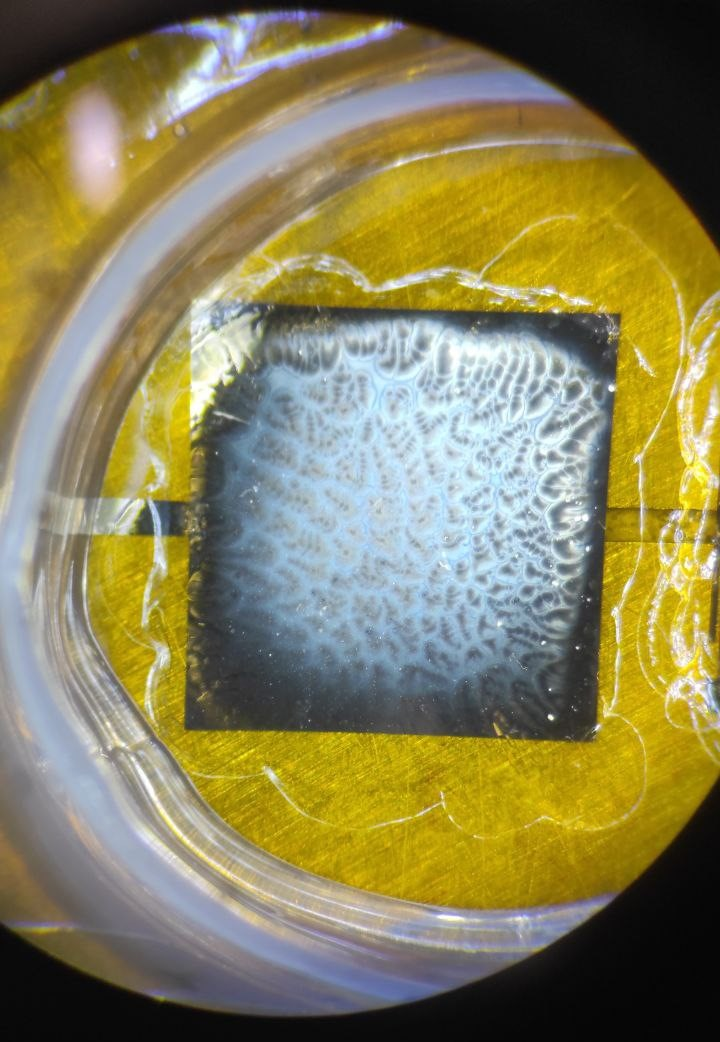
\includegraphics[width=0.3\textwidth]{figures/chapter4/ammonium/gate_membrane.jpg}}
    \caption{Optical image of the ion-sensitive membrane deposited on the gate electrode.}
    \label{fig:ammoniumMembrane}
\end{figure}

In the previous section I demonstrated that I fabricated a stable EG-CNTFET transducer that I can use for a (bio)sensor, based on the standard EG-FET geometry. In this chapter I am going to illustrate the results of a sensor built with such technology.

As a result of the previous work, the functionalization of the CNTs is off-limits, and it remains possible to functionalize the gate. This opens up many possibilities for functionalization, as explained in the introductory section, especially in terms of covalent and stable functionalization that does not interfere with the mobility of the semiconductor. With this in mind, the gate was first functionalized with an ion-selective membrane containing nonactin, as described in section \ref{sec:materials}, which is sensitive to ammonium ions. This membrane is also PVC-based, like the lipophilic membrane on the channel, but it dries differently, resulting in translucency and opacification of the underlying gate, as can be seen in Figure \ref{fig:ammoniumMembrane}.

Once deposited and allowed to dry in an overnight refrigerated environment, the membrane had to have been conditioned 24 hours in 1X PBS containing \SI{1}{mM} ammonium; the reason for the conditioning is not entirely clear; it can be speculated that priming of the ionophore plays an important role, together with the absorption of water molecules, primary and interfering ions \citep{petrelliMethod2023}. \citet{petrelliMethod2023} showed that without this step the sensitivity of the sensor decreases significantly and therefore it is advisable to perform this step.
After conditioning, electrical characterization was performed by first collecting transfer characteristics. The device was allowed to stabilize in 1X PBS for 60 min, after which 5 injections of increasing concentrations of ammonium from 0.01 to 100mM were made, one every 10 min. At the end of the collection, the \ion{} was extracted, with the result shown in Figure \ref{fig:normTransferAmm}. For each injection, the current of the last 4 points was averaged, the standard deviation was calculated, and the result can be seen in Figure \ref{fig:calTransferAmm}. It can be seen that for this type of experiment, the measurements obtained in this way led to an illegible result, in which a difference in current between the first 4 injections is hardly visible and the last one even results at a much lower current, contrary to expectation.

\begin{figure}[]
    \centering
    \subfloat[$\mathrm{I_{ON}^*}$]{%
        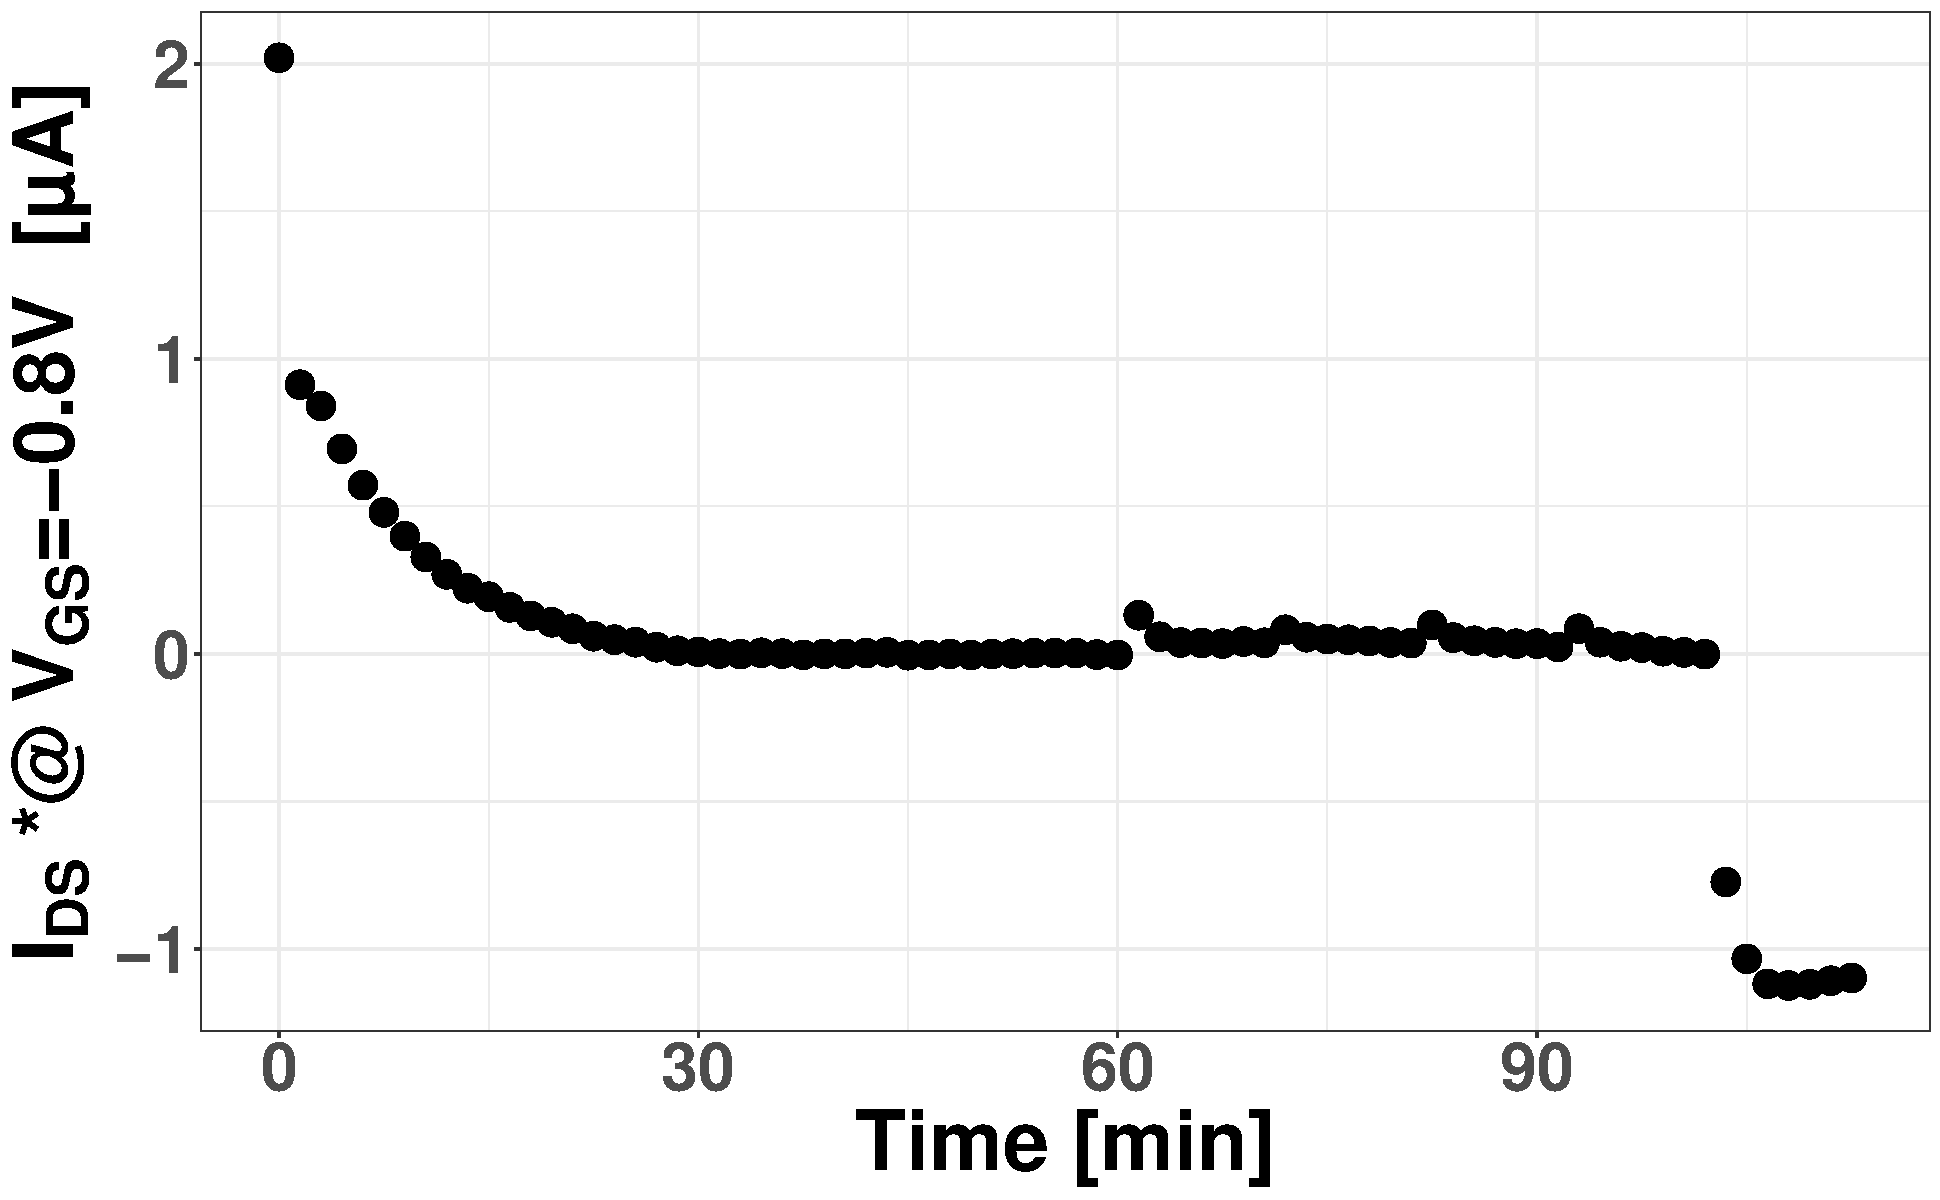
\includegraphics[width=0.45\textwidth]{figures/chapter4/ammonium/correctedPlot_transfers.pdf}
        \label{fig:normTransferAmm}
    }
    \hfill
    \subfloat[Calibration plot]{%
        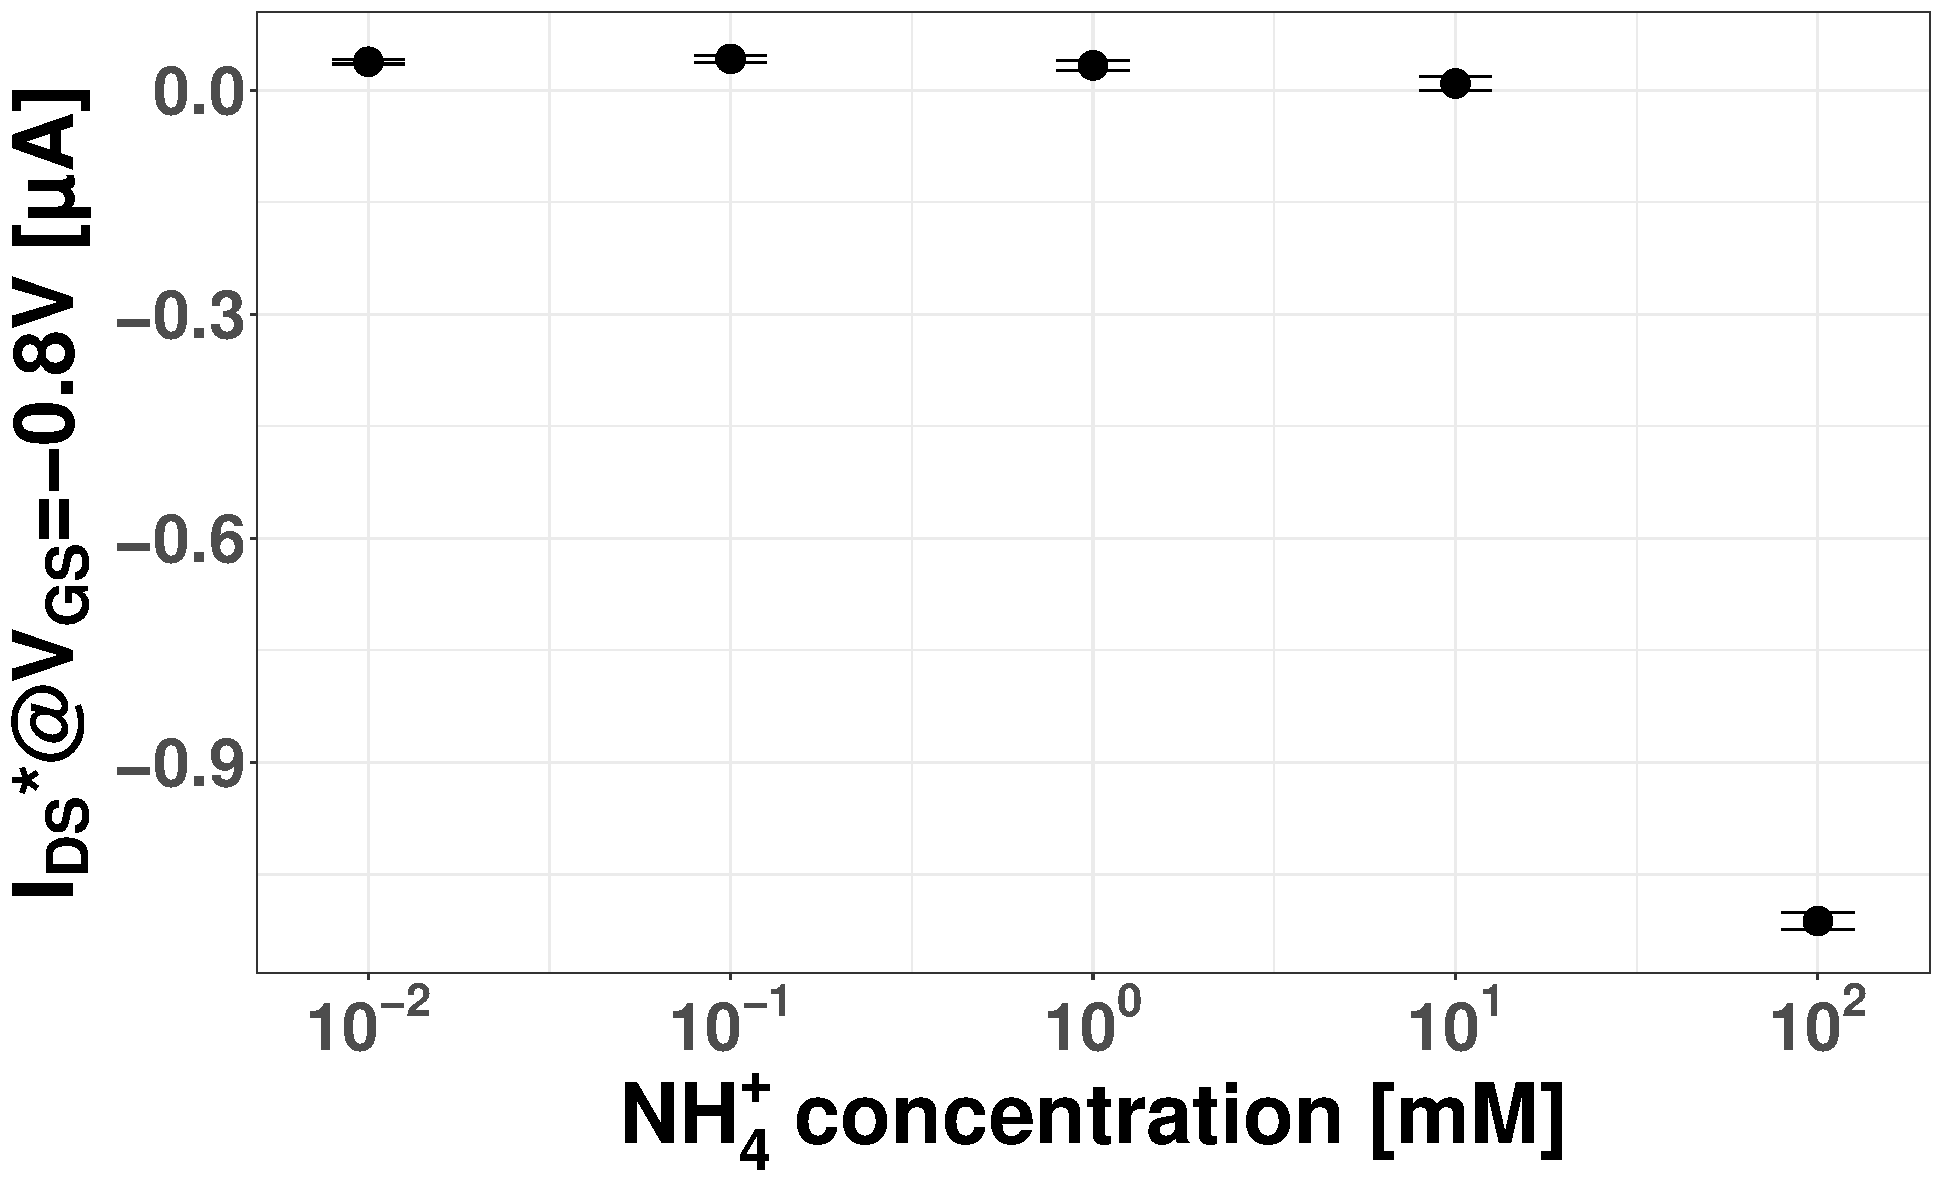
\includegraphics[width=0.45\textwidth]{figures/chapter4/ammonium/calibrationPlot_transfers.pdf}
        \label{fig:calTransferAmm}
    }
    \caption{Electrical characterization of the biosensor: 40 transfer characteristics were collected over the span of \SI{60}{\min} to let the devices stabilize; after this time, 5 increasing concentrations of \amm{} were injected every \SI{10}{\min} (7 transfer curves). The \ion{} was extracted for each curve, the linear fitting calculated over the last 30 minutes of stabilization and the baseline removed, as to obtain the corrected ON current ($\mathrm{I_{ON}^*}$).
    (a) \ioncorr{}. The injection moments are visible as small peaks in the signal.
    (b) Calibration curve obtained by averaging the last four data points of the \ioncorr{} for each concentration. The resulting trend does not match expectations, indicating the need for an alternative measurement or analysis strategy.}
    \label{fig:transferAmm}
\end{figure}

Therefore, the strategy was revised and a new protocol was developed: the experiment was conducted with chronoampetrometry measurements, in which both \vds{} and \vgs{} were fixed and the current was measured over time. In Figure \ref{fig:normChronoAmm} it can be seen how the signal of the injections is much more visible and how they drastically affect the system, which then returns to equilibrium; this is demonstrated by the fact that the current (in modulus) increases very rapidly and very violently after each injection, and then drops and returns to the initial intensity. The calibration plot (Figure \ref{fig:calChronoAmm}) was made in this case by calculating the mean and standard deviation of the current measured during the last 5 minutes of each injection. In this it is possible to observe the expected behavior, \ie{} the signal increases linearly in response to increasing concentrations of analyte, with a sensitivity of \SI{0.14}{\uA \per decade} and a coefficient of determination of 0.94. Thus, it is possible to conclude that an ammonium ion sensor was successfully fabricated using a stable EG-CNTFET as the transducer.

\begin{figure}
    \centering
    \subfloat[Normalized current]{
        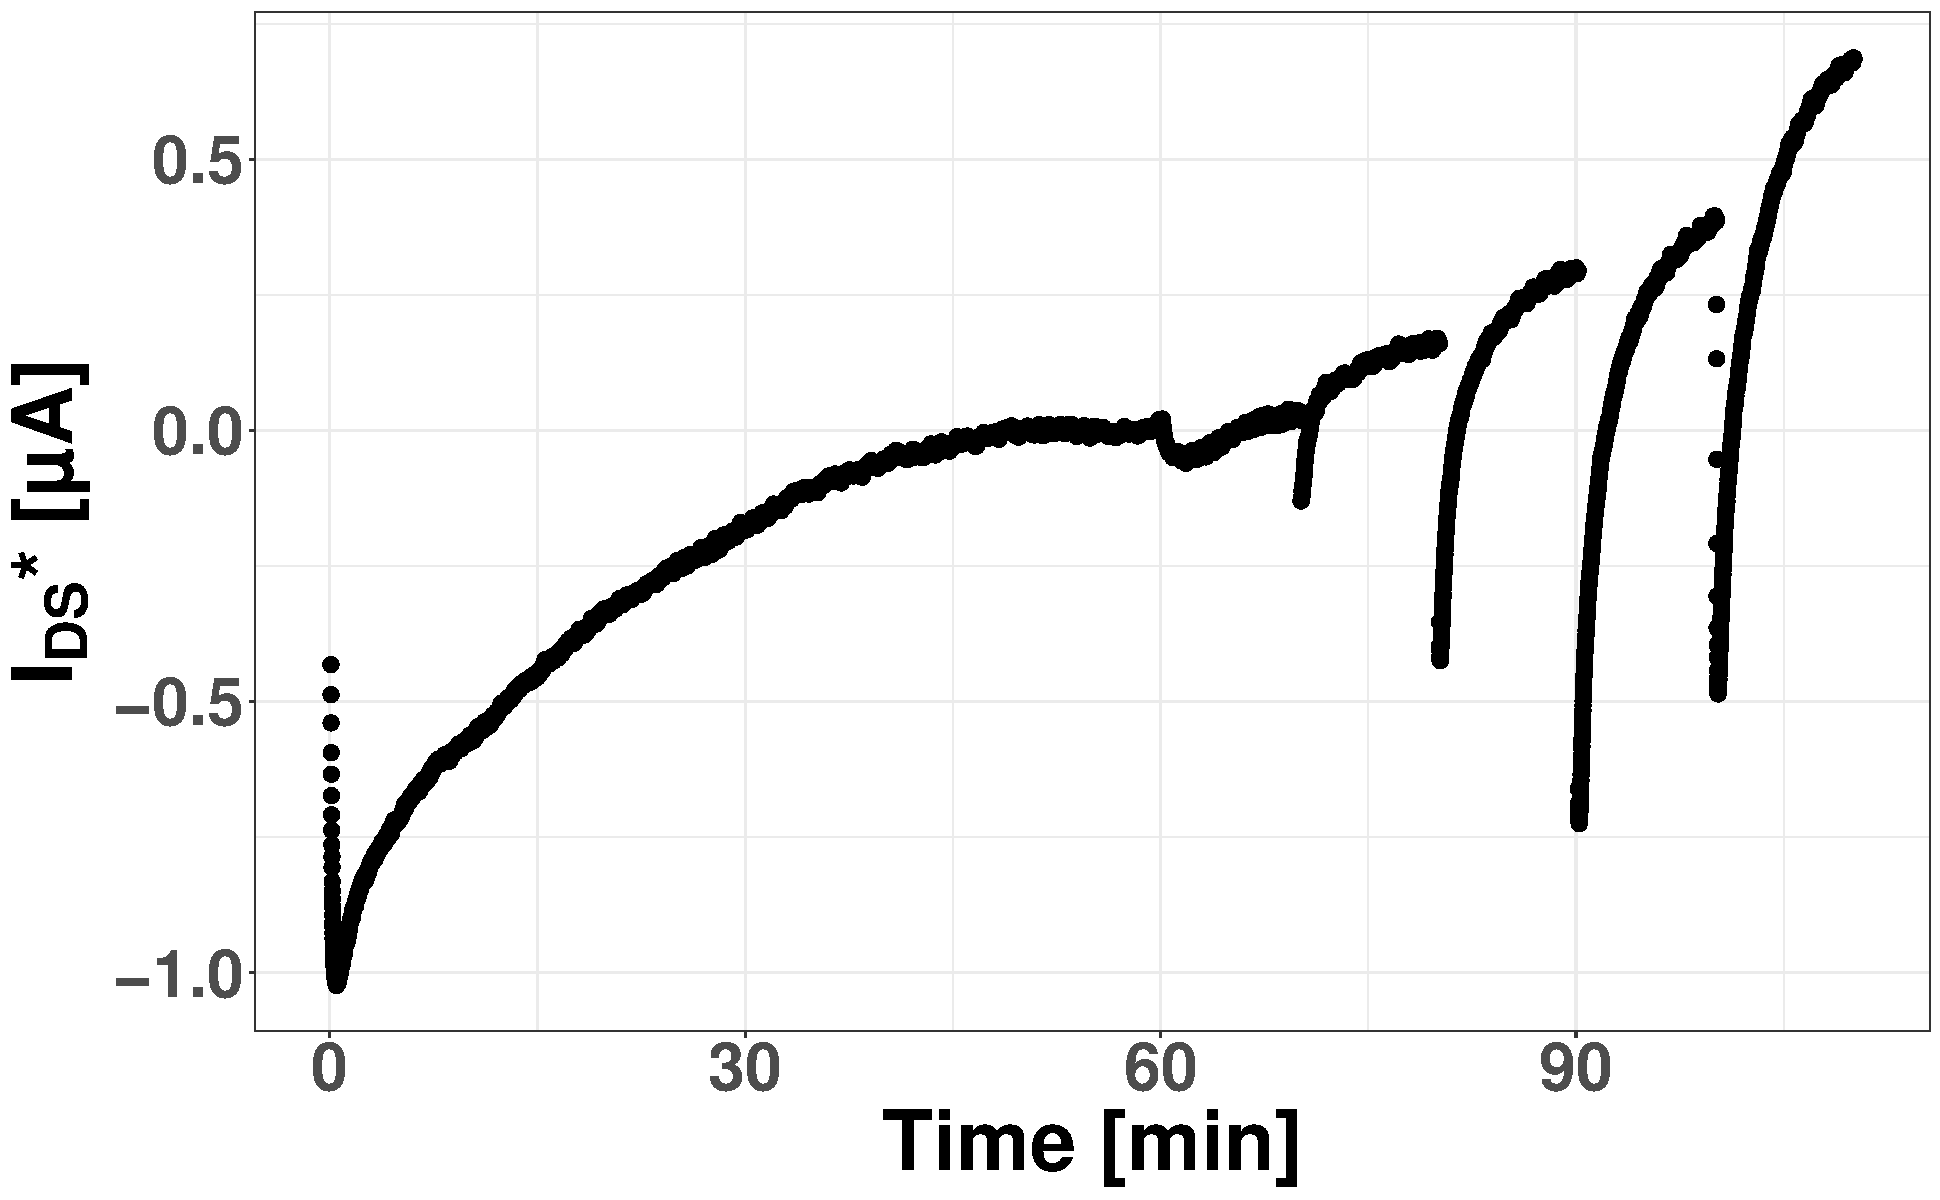
\includegraphics[width=0.45\textwidth]{figures/chapter4/ammonium/correctedPlot-chronoamperometry.pdf}
        \label{fig:normChronoAmm}
    }
    \hfill
    \subfloat[Calibration plot]{
        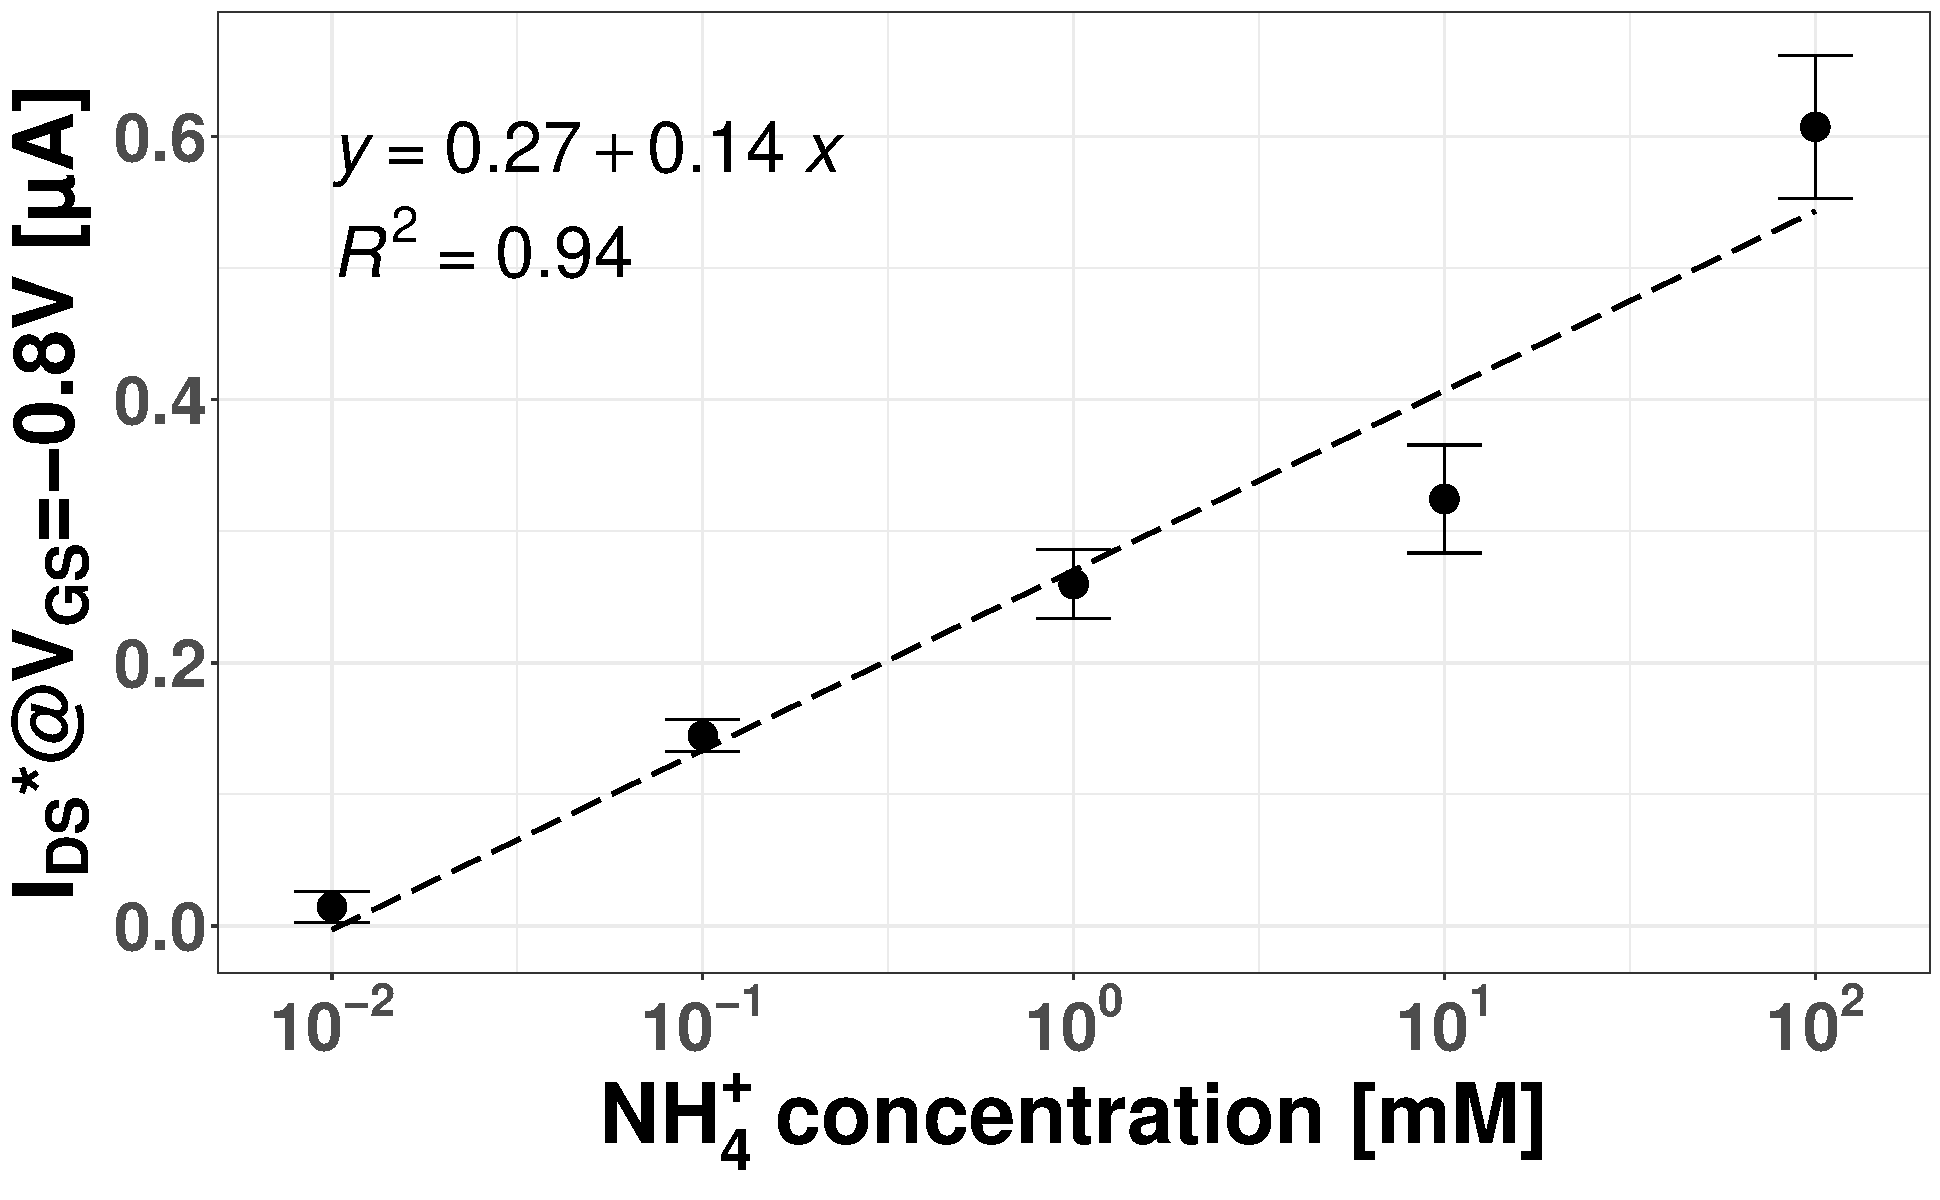
\includegraphics[width=0.45\textwidth]{figures/chapter4/ammonium/calibrationPlot-chronoamperometry.pdf}
        \label{fig:calChronoAmm}
    }
    \caption{Electrical characterization of the biosensor through chronoamperometric measurements: both the \vds{} and \vgs{} and the response of the device was taken over time. The current was fitted with a linear model from \SIrange{30}{60}{\min} and the baseline removed to obtain a corrected current (\idscorr{})
    (a) \idscorr{} over time during chronoamperometric measurements. Injection moments appear as small peaks in the current. 
    (b) Calibration plot obtained by averaging the final four points of the \idscorr{} at each concentration. The linear detection range for \amm{} falls between \SIrange{0.01}{100}{mM}, with a sensitivity of \SI{0.14}{\uA \per decade} and a \rsq{}$= 0.94$.}
    \label{fig:sensing_chronoamperometry}
\end{figure}

